\chapter{Meetresultaten}%
\label{ch:benchmarks}

De performantie van \textit{WebGPU} in vergelijking met andere technologieën kan sterk verschillen. Om een beeld te vormen over de capaciteiten die \textit{WebGPU} brengt, worden in dit hoofdstuk enkele testen uitgevoerd. Hierdoor kan er vergeleken worden hoe de prestaties van \textit{WebGPU} al dan niet overeenstemmen met traditionele \textit{GPGPU} technologieën zoals \textit{CUDA}, of normale rekenkracht beschikbaar gesteld door een \textit{Central Processing Unit} (\textit{CPU}).

\section{Transformer prestaties van WASM en WebGPU}

Een andere opkomende technologie is \textit{web assembly} (\textit{WASM}). \textit{WASM} is een zeer compact \textit{assembly-like binary} die performantie toelaat vergelijkbaar met \textit{native} talen zoals \textit{C/C++} en \textit{Rust}~\autocite{Steiner2023}.

\begin{displayquote}[{\cite{Chen2020}}]
    "We introduced support for WASM and WebGPU backends to the Apache TVM deep learning compiler. Our initial experiments shows that TVM's WebGPU backend can get close to native GPU performance when deploying models in the browser."
\end{displayquote}

Deze \textit{low-level} programmeertalen laten, net zoals \textit{WGSL} voor \textit{WebGPU} toe, dat rekenkundige taken optimaal worden uitgevoerd. Dit komt omdat de code specifiek wordt geschreven op een manier die rekening houdt met hoe de onderliggende hardware functioneert~\autocite{Knight2020}.

\begin{figure}
    \centering
    \pgfplotsset{width=15cm,compat=1.9}

% We will externalize the figures
% \tikzexternalize
\pgfplotsset{
  log ticks with fixed point,
}
\begin{tikzpicture}
    \begin{semilogxaxis}[
        title={Transformer benchmark fp32 WASM versus WebGPU},
        xlabel={Batch size},
        ylabel={Uitvoeringstijd in ms},
        xmin=1, xmax=64,
        ymin=0, ymax=70000,
        xtick={1,2,4,8,16,32, 64},
        ytick={1,10000,20000,30000,400000,50000,60000, 70000},
        legend pos=north west,
        ymajorgrids=true,
        grid style=dashed,
        scatter/classes={
            a={mark=square*,red},
            b={mark=triangle*,orange},
            c={mark=o,draw=blue},
            d={mark=square,green}
        },
        yticklabel style={
            /pgf/number format/fixed,
        },
        scaled y ticks=false
    ]
    
        \addplot[
            color=red,
            mark=square*
            ]
            coordinates {
                (1, 946.14)(2, 1923.12)(4, 3816.90)(8, 7653.00)(16, 15494.62)(32, 30901.40)(64, 61788.00)
            };
            \addlegendentry{WASM (fp32) Intel Xeon E5-2680 V2}
            
        \addplot[
            color=orange,
            mark=triangle*
            ]
            coordinates {
                (1, 747.10)(2, 1499.98)(4, 3014.38)(8, 5956.38)(16, 11807.70)(32, 24121.56)(64, 47769.14)
            };
            \addlegendentry{WASM (fp32) Intel Core i9-9980HK}
        \addplot[
            color=blue,
            mark=o
            ]
            coordinates {
                (1, 193.66)(2, 365.90)(4, 703.24)(8, 1393.12)(16, 2752.66)(32, 5510.74)(64, 10966.04)
            };
            \addlegendentry{WebGPU (fp32) Intel UHD Graphics 630}

        \addplot[
            color=green,
            mark=square
            ]
            coordinates {
                (1, 28.02)(2, 58.28)(4, 77.74)(8, 116.40)(16, 226.00)(32, 463.16)(64, 739.16)
            };
            \addlegendentry{WebGPU (fp32) Nvidia Geforce GTX 1080 Ti}
        \addplot [
            scatter,only marks,
            scatter src=explicit symbolic,
        ] table [x=x,y=y,meta=label] {plotdata/HuggingFaceWasmVSWebGPU.dat};

    \end{semilogxaxis}
\end{tikzpicture}
\end{figure}
\label{sec:transformerbench}

\subsection{Uitvoeren van de test}

De performantie van verschillende testopstellingen werd opgemeten aan de hand van de \textit{webgpu-embedding-benchmark} van \textcite{Lochner2024}. Hierbij blijkt \textit{WebGPU} consistent sneller dan \textit{WASM} voor zowel sterke als zwakke grafische kaarten. In deze test werd de uitvoeringstijd gemeten van \textit{BERT-based embedding} modellen met zowel \textit{WebGPU} als \textit{WASM}, en dit telkens voor een toenemende \textit{batch size}.

\bigbreak{}

Voor een \textit{batch-size} van 64 doet de \textit{Xeon E5-2680 V2} gemiddeld 60 seconden over de \textit{transformer} test. Wanneer deze tijd als basis wordt genomen is de \textit{Intel Core i9-9980HK 10} seconden sneller.

\subsection{Vergelijken van resultaten}

Een veel gebruikte standaard om rekenkracht van computer onderdelen te vergelijken is door het aantal berekeningen van comma getallen per seconden op te meten. Deze berekening wordt uit gedrukt in \emph{floating point operations per second} (\textit{FLOPS}) en laat dus toe om algemene rekenkracht van verschillende componenten te vergelijken. 

\bigbreak{}

Zowel theoretische waarden als meetresultaten werden telkens vergeleken met de \textit{base line} gebaseerd op de performantie van de \textit{Xeon E5-2680 v2}. Bij het uitvoeren van deze testen werd de sequentie lengte steeds ingesteld op 512. Deze lengte beschrijft het aantal \textit{tokens} die samen worden gegroepeerd door de \textit{transformer}. Ook werden alle testen uitgevoerd met \emph{Chrome versie 124}.

\break{}

\begin{table}[t]
    \begin{tabular}{ |p{5.5cm}|p{2.5cm}|p{2.5cm}|p{3.5cm}|  }
        \hline
        \multicolumn{4}{|c|}{Vergelijken van theoretische \textit{Floating Point} prestaties met meetresultaten} \\
        \hline
        Component& Theoretisch GFLOPS & Theoretisch vergelijking & Resultaten transformertest\\
        \hline
            Xeon E5-2680 V2             & 224,0     & 100\%  & 100\%       \\
            Intel Core i9-9980HK        & 307,2     & 137\%  & 129\%    \\
            Intel UHD Graphics 630      & 403,2     & 180\%  & 560\%    \\
            Nvidia GeForce GTX 1080 Ti  & 11.340,0  & 5063\% & 7170\%   \\
        \hline
    \end{tabular}
    \caption[\textit{Floating point} performantie \textit{CPU's} en \textit{GPU's} \autocite{Intel2024, Intel2024a, TechPowerUp2017, TechPowerUp2017a}]{Theoretische floating point performantie \autocite{Intel2024, Intel2024a, TechPowerUp2017, TechPowerUp2017a}}
    \label{tab:TheoreticalVersusMeasuredPerf}
\end{table}

In tabel \ref{tab:TheoreticalVersusMeasuredPerf} werd de \textit{Xeon E5-2680 v2} als basis gebruikt om de andere componenten te vergelijken. Omdat de \textit{Intel Core i9-9980HK} een nieuwere processor is, is deze gemiddeld voor alle \textit{batch} groottes 29\% sneller. Ook werd de theoretische snelheid van deze componenten opgenomen in deze table zodat er kan vergeleken worden of de meetresultaten overeen komt met wat theoretisch verwacht wordt van de individuele componenten. 

\bigbreak{}

Voor de processoren werd de \textit{Intel} specificatie gebruikt om de theoretische \textit{GFLOPS} te bepalen~\autocite{Intel2024, Intel2024a}. De \textit{GFLOPS} voor de grafische kaarten werd gebaseerd op informatie die beschikbaar werd gesteld door \textcite{TechPowerUp2017, TechPowerUp2017a}.

\subsection{Conclusie}

Uit de grafiek en de tabel valt af te leiden dat voor deze test \textit{WebGPU} een geschikte technologie is voor het trainen van AI-modellen op de browser. De test duidt ook aan dat het inzetten van de grafische kaart voor deze \textit{embedding} berekeningen een geschiktere component is dan een processor implementatie.

\bigbreak{}

Ook valt af te leiden uit de resultaten van de \textit{Embedding Benchmark} van \textcite{Lochner2024} dat \textit{WebGPU} beter presteert dan verwacht uit de theoretische snelheden. Dit ligt aan de implementatie van de test. Net zoals \textit{WebGPU} is \textit{WebAssembly} een nieuwe technologie. Beide technologieën zijn nog in ontwikkeling en kunnen verder verbeterd worden. Dit blijkt ook uit de testen die in sectie \ref{sec:whispertest} werden uitgevoerd. De resultaten van de \textit{WASM} testen liggen dichter bij de theoretische verwachtingen. Dit wijst erop dat de \textit{WASM} implementaties onderpresteren maar wel correct schalen bij krachtigere processoren. Hierdoor lijken de \textit{WebGPU} resultaten een stuk beter dan wat theoretisch verwacht werd.

\break{}

\section{Whisper implementaties met CPU, \textit{CUDA} en WebGPU}%
\label{sec:whispertest}

Het Whisper AI-model van \textcite{OpenAI2023} wordt online gepubliceerd met verschillende parameter groottes. Een model neemt steeds meer geheugen in naarmate het aantal parameters stijgt en er geen optimalisaties worden uitgevoerd. Hierdoor kan met deze modellen goed getest worden omdat de prestaties beïnvloed worden door het aantal parameters. Er geldt wel een begrenzing voor apparaten met beperkt geheugen. Niet alle apparaten hebben namelijk evenveel beschikbaar geheugen, en kunnen dus niet alle Whisper modellen uitvoeren. 

\bigbreak{}

Grafische kaarten laten niet enkel hoge parallellisatie toe, maar hebben in het algemeen ook een veel hogere geheugenbandbreedte dan het RAM-geheugen van een processor zie tabel \ref{tab:RAMSpeeds}. Deze bandbreedte speelt ook een rol bij het uitvoeren van inferentie, en heeft dus effect op hoe snel het \textit{Whisper} model een audio fragment kan interpreteren.

\bigbreak{}

\textit{Whisper} kan als module in \textit{Python} worden geïmporteerd. Door een testscript te schrijven kunnen verschillende modelgroottes worden ingeladen. Dit script kan worden teruggevonden in de bijlage sectie \ref{sec:whispertestcode}. Ook laat de \textit{Whisper} module in \textit{Python} toe om alsnog de CPU te gebruiken. Wanneer \textit{torch} wordt geïnstalleerd voor \textit{Python} kan deze ook worden ingesteld om gebruik te maken van \textit{CUDA}. Hierna kan de \textit{Whisper} module het \textit{CUDA} apparaat gebruiken op \textit{Python}. \textit{WebGPU} kon getest worden met Whisper omwille van de implementaties van \textcite{Fleetwood2024, Fleetwood2023b}.

\bigbreak{}

De modellen van OpenAI met verschillende parametergroottes zijn beschikbaar op \href{https://github.com/openai/whisper}{GitHub.com/OpenAI/Whisper}. De modellen die zijn opgelijst in tabel \ref{tab:OpenAIWhisperModels}, werden allemaal getest met \textit{CUDA} en processor implementaties in \textit{Python}. De base, small en large modellen werden getest met WebGPU.

\begin{table}[b]
    \begin{tabular}{ |p{1.6cm}|p{2.5cm}|p{2.7cm}|p{2.7cm}|p{1.9cm}|p{1.8cm}|  }
        \hline
        \multicolumn{6}{|c|}{Beschikbare modellen en talen Whisper} \\
        \hline
            Grootte& Parameters & English-only model & Multilingual model & Vereiste VRAM & Relatieve snelheid\\
        \hline
            tiny&       39 M    &tiny.en    & tiny& ~1 GB& ~32x     \\
            base &      74 M	&base.en    & base & ~1 GB & ~16x   \\
            small &     244 M	&small.en   & small & ~2 GB & ~6x   \\
            medium &    769 M	&medium.en  & medium & ~5 GB & ~2x  \\
            large &     1550 M	&N/A        & large & ~10 GB& 	1x  \\
        \hline
    \end{tabular}
    \caption{Whisper modellen beschikbaar gesteld door \textcite{OpenAI2023}.}
    \label{tab:OpenAIWhisperModels}
\end{table}

\break{}

\subsection{Uitvoeren van Python testscript}

Omdat Whisper zoveel verschillende modelgroottes beschikbaar stelt maakt dit het AI-model zeer geschikt om te testen met \textit{WebGPU}, maar ook met \textit{CUDA} en normale processor implementaties. Door verschillende grafische kaarten en processoren te testen kon hierdoor een beeld gegeven worden wat de verwachte prestaties zijn die \textit{WebGPU} kan bieden in vergelijking met normale processoren of geavanceerdere \textit{CUDA} implementaties. De invloed van de toenemende parametergrootte op de uitvoeringstijd kan hierdoor ook duidelijk worden gerepresenteerd.

\bigbreak{}

Om testresultaten op een consistente manier te verzamelen werd een \textit{Python} script geschreven. Dit script werd dan op verschillende apparaten uitgevoerd om op deze manier betrouwbare data te verzamelen. Er werd telkens gebruik gemaakt van \textit{Python} versie 3.11, in combinatie met \textit{torch} en \textit{torchaudio} versie 2.0.0+cu117 en \textit{torchvision} versie 0.15.0+cu117.

\bigbreak{}

Om de prestaties van \textit{WebGPU} te onderzoeken werd de implementatie van \textcite{Fleetwood2024} gebruikt. Deze geeft namelijk telkens de inferentie tijd weer, die nodig was voor het uitvoeren. Deze data werd manueel verzameld.

\bigbreak{}

\subsection{Installatie afhankelijkheden}

Om \textit{Whisper} operationeel te krijgen op een \textit{Windows 10} installatie zijn er verschillende afhankelijkheden die moeten worden geïnstalleerd. Dit betreft \textit{Python 3.9.9}, \textit{PyTorch 1.10.1} en de \textit{CUDA toolkit}. Het is ook belangrijk op te merken dat \textit{torch} moet worden gecompileerd met \textit{CUDA} functionaliteit, indien dit niet wordt gedaan, kan enkel door middel van de processor de \textit{Whisper} modellen worden uitgevoerd.

\subsection{Opzetten van de test}

Zowel \textit{Windows 10} als \textit{Ubuntu server 22.04} werden getest met versies van \textit{Whisper} ondersteund door \textit{CUDA} en \textit{CPU}. Maar om de performantie van \textit{WebGPU} te kunnen vergelijken met \textit{CUDA} werd enkel op \textit{Windows 10} getest met een \textit{Nvidia GeForce GTX 1080 Ti} grafische kaart. Hierdoor kon consistente data verzameld worden.

\break{}

% PS > pip3 uninstall torch torchvision==0.15.0 torchaudio==2.0.0
% PS > pip3 cache purge
% PS > pip3 install torch torchvision==0.15.0 torchaudio==2.0.0 --index-url https://download.pytorch.org/whl/cu117

% import torch
% torch.cuda.is_available()
% # returns False
% torch.zeros(1).cuda()
% # throws AssertionError: Torch not compiled with CUDA enabled

% \begin{lstlisting}[language=Python]
% import torch
% torch.cuda.is_available()
% # returns True
% torch.zeros(1).cuda()
% # returns tensor([0.], device='cuda:0')
% \end{lstlisting}
\begin{figure}
    \centering
    \pgfplotsset{width=15cm,compat=1.9}

\pgfplotsset{
  log ticks with fixed point,
}

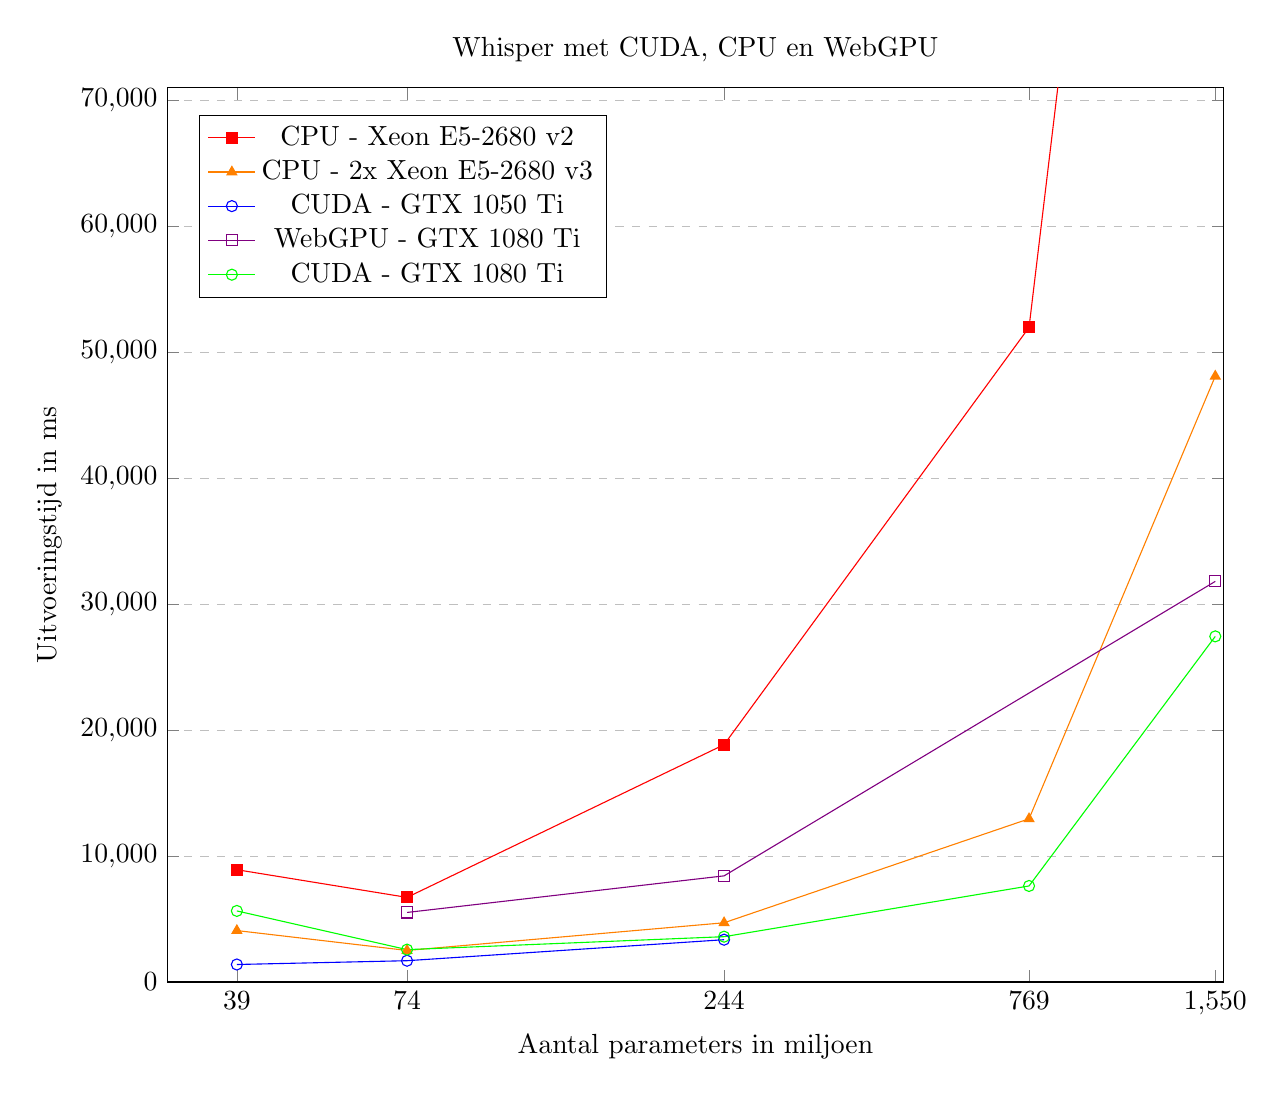
\begin{tikzpicture}
    \begin{semilogxaxis}[
        title={Whisper met CUDA, CPU en WebGPU},
        xlabel={Aantal parameters in miljoen},
        ylabel={Uitvoeringstijd in ms},
        xmin=30, xmax=1600,
        ymin=0, ymax=71000,
        xtick={39, 74, 244, 769, 1550},
        legend pos=north west,
        ymajorgrids=true,
        grid style=dashed,
        yticklabel style={
            /pgf/number format/fixed,
        },
        scaled y ticks=false
    ]
    \addplot[
            color=red,
            mark=square*
        ]
        coordinates {(39,8919)(74,6721)(244,18849)(769,51980)(1550,175378)};
        \addlegendentry{CPU - Xeon E5-2680 v2}

    \addplot[
        color=orange,
        mark=triangle*
        ]
        coordinates {(39,4088)(74,2508)(244,4706)(769,12963)(1550,48107)};
        \addlegendentry{CPU - 2x Xeon E5-2680 v3}

    \addplot[
            color=blue,
            mark=o
        ]
        coordinates {(39,1393)(74,1694)(244,3362)};
        \addlegendentry{CUDA - GTX 1050 Ti}
    
    \addplot[
            color=violet,
            mark=square
        ]
        coordinates {(74,5526)(244,8431)(1550,31814)};
        \addlegendentry{WebGPU - GTX 1080 Ti}

    \addplot[
            color=green,
            mark=o
        ]
        coordinates {(39,5647)(74,2574)(244,3602)(769,7629)(1550,27448)};
        \addlegendentry{CUDA - GTX 1080 Ti}
    \end{semilogxaxis}
\end{tikzpicture}
\end{figure}

% pip3 install torch torchvision==0.15.0 torchaudio==2.0.0 --index-url https://download.pytorch.org/whl/cu117
% pip3 install torch torchvision==0.15.0 torchaudio==2.0.0 --index-url https://download.pytorch.org/whl/cpu
% pip3 uninstall torch torchvision==0.15.0 torchaudio==2.0.0
% pip3 cache purge

\subsection{Resultaten van de Whisper test}

Uit de resultaten kan worden afgeleid dat zelfs krachtige processoren zoals de Xeon E5-2680 v2 en v3 al snel niet op kunnen tegen de parallelle rekenkracht van grafische kaarten. De experimentele \textit{WebGPU} implementatie van \textcite{Fleetwood2024} kan niet evenaren aan de \textit{CUDA} implementatie, deze verschillen gemiddeld 53,4\%, 57,2\% en 13,7\% bij respectievelijk de \textit{base}, \textit{small} en \textit{large} implementaties van \textit{Whisper}. Relatief gezien ten opzichte van de processor prestaties van de \textit{Xeon E5-2680 v2} is dit geen groot verschil, omdat deze processor prestaties naarmate dat het \textit{Whisper} model wordt uitgevoerd met toenemende parameter grootte niet goed schaalt.

\bigbreak{}

Het is wel belangrijk te vermelden dat bij de \textit{large} implementatie van \textit{Whisper} het \textit{VRAM} geheugen gebruik van het model substantieel lager was in \textit{WebGPU} dan in de \textit{CUDA} implementatie en dat hierdoor het model mogelijks een andere kwantisatie wordt toegepast. Dit kan leiden tot een verlaagd \textit{VRAM} gebruik.

\bigbreak{}

Initieel presteren de twee \textit{Xeon E5-2680 v3} processoren beter dan de \textit{WebGPU} implementatie. Maar naarmate het model in parameter grootte toeneemt wordt duidelijk dat de uitvoeringstijd sterk begint te stijgen. De verhoogde parallelle rekenkracht van de grafische kaarten zijn hiertegen beter opgewassen. Ook speelt de verhoogde \textit{VRAM} bandbreedte hier een rol. Het verschil in RAM bandbreedte van de processoren en grafische kaarten kan worden vergeleken in table \ref{tab:RAMSpeeds}. 

\bigbreak{}

Omwille van het beperkte geheugen waarover de \textit{GTX 1050 Ti} beschikt (4GB) kon deze enkel worden getest tot en met het kleine \textit{Whisper} model (244 miljoen parameters). Dit is een belangrijke beperking om in acht te houden bij gebruiken grafische kaarten voor de uitvoering van AI-modellen. Wanneer \textit{WebGPU} of \textit{CUDA} technologie wordt gebruikt om AI-modellen uit te voeren moet er rekening worden gehouden hoeveel beschikbaar werkgeheugen er is. Wanneer deze grens wordt bereikt, wordt vaak het gedeelde geheugen gebruikt. Hierdoor wordt de bandbreedte sterk beperkt omdat er een constante uitwisseling moet plaats vinden tussen het geheugen van de grafische kaart en het geheugen van de processor.

\subsection{Conclusie}

De \textit{Xeon} processoren die gebruikt werden voor deze test zijn niet representatief voor een eindgebruiker. Deze processor opstelling vertegenwoordigd een traditionele server implementatie. Het is belangrijk om op te merken dat processoren van de eindgebruiker meestal niet kunnen evenaren aan deze processor prestaties. Deze Xeon processoren werden getest om een vergelijking te maken met hoe het \textit{Whisper} model kan worden geïmplementeerd aan de server kant, en welke prestaties hierbij kunnen worden verwacht. Er kan namelijk niet realistisch worden verwacht van eindgebruikers om complexe software zoals CUDA te installeren zodat het Whisper model kan worden gebruikt. Daarom zou deze implementatie moeten worden uitgevoerd op een server waarop een eindgebruiker dan toegang tot heeft.

\bigbreak{}

Performante grafische kaarten daarentegen zijn wel beschikbaar voor de eindgebruiker omwille van de proliferatie van videogames. Een implementatie van het \textit{Whisper} model op de browser kan zeker voordelen geven wanneer deze gebruik kan maakt van lokale componenten. Ook laat het lokaal verwerken van audio een verhoogde privacy toe voor de eindgebruiker. En wanneer een webapplicatie die het \textit{Whisper} model lokaal implementeert wordt omgevormd tot een \textit{PWA} kan deze zelf offline gebruikt worden.

\begin{table}[b]
    \begin{tabular}{ |p{5.3cm}|p{2.9cm}|p{3.0cm}|p{2.7cm}|  }
        \hline
        \multicolumn{4}{|c|}{\textit{Random Access Memory} snelheden} \\
        \hline
        Component& DDR generatie & Klokfrequentie & Bandbreedte \\
        \hline
            Xeon E5-2680 V2             & DDR 3     & 1866 MHz  & 59.7 GB/s \\
            2x Xeon E5-2680 V3          & DDR 4 ECC & 2133 MHz  & 136 GB/s  \\
            Nvidia GeForce GTX 1050 Ti  & GDDR 5    & 7008 MHz  & 112.1 GB/s\\
            Nvidia GeForce GTX 1080 Ti  & GDDR 5X   & 11000 MHz & 484.4 GB/s\\
        \hline
    \end{tabular}
    \caption[Verschillen in RAM snelheden voor \textit{CPU's} en \textit{GPU's}~\autocite{Intel2013,Intel2014,TechPowerUp2016, TechPowerUp2017}]{\textit{Random Access Memory} snelheden van \textit{CPU's} volgens \textcite{Intel2013,Intel2014} en \textit{GPU's} volgens \textcite{TechPowerUp2016, TechPowerUp2017}}
    \label{tab:RAMSpeeds}
\end{table}
